\scanpage{35}
(1.8) Considérons enfin les p\textsuperscript{ts} fixes
\[
(32)\qquad\deleted{\unsure{\beta_0}}\inserted{\alpha'(0)}=2,\quad
\deleted{\unsure{\beta_1}}\inserted{\alpha'(1)}=-1,\quad
\deleted{\unsure{\beta_\infty}}\inserted{\alpha'(\infty)}=\frac12
\]
\figure{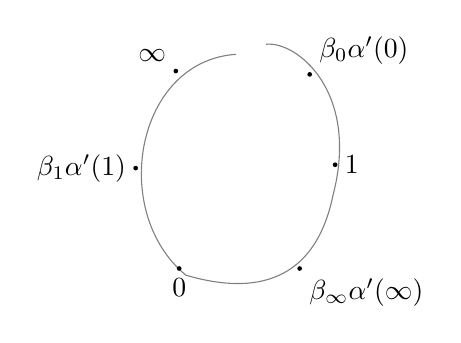
\begin{tikzpicture}[scale=.85]
\draw[gray] (0,1.65).. controls(-1.5,1.55) and(-1.9,-.7)..(-.75,-1.65)
.. controls(.1,-1.9) and(1.15,-1.9)..(1.45,-.45)
.. controls(1.85,1.1) and(.9,1.85)..(.45,1.8);
\foreach \x/\y in {-.9/1.4,1.1/1.35,1.48/0,.95/-1.55,-.85/-1.55,-1.5/-.05}
\fill (\x,\y) circle(.035);
\node[above left] at(-.9,1.4){$\infty$};
\node[above right] at(1.1,1.35){$\deleted{\unsure{\beta_0}}\inserted{\alpha'(0)}$};
\node[right] at(1.48,0){$1$};
\node[below right] at(.95,-1.55){$\deleted{\unsure{\beta_\infty}}\inserted{\alpha'(\infty)}$};
\node[below] at(-.85,-1.55){$0$};
\node[left] at(-1.5,-.05){$\deleted{\unsure{\beta_1}}\inserted{\alpha'(1)}$};
\end{tikzpicture}}
qui sont les p\textsuperscript{ts} fixes, autres que $0,1,\infty$ resp., des
transpositions $\tau_0$, $\tau_1$, $\tau_\infty\in\unsure{\mathfrak S_3|\mathbb G_3}$.
soit
\figure{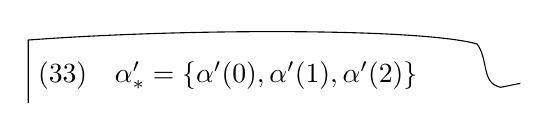
\begin{tikzpicture}
\node[anchor=west] at(0,0){$(33)\quad\alpha'_*=
\{\alpha'(0),\alpha'(1),\alpha'(2)\}$};
\draw (0,-.35)--(0,.45).. controls(2,.6) and(5,.6)..(5.7,.4)
.. controls(5.85,.2) and(5.75,-.1)..(6,-.15)--(6.25,-.1);
\end{tikzpicture}}
On veut déterminer $E(\alpha'_*)$ \inserted{$=\coprod_{i\in I}E(\alpha'(i))$}
comme $\mathcal E$-ensemble.
On trouve
\[
(34)\qquad\left\{\begin{aligned}
E_n(\alpha'(i))&\simeq\{(\zeta_j)\in\overline{\mathbb Q}^{\,I\setminus\{i\}}
\mid\zeta_j^{\unsure{n}}=-\tfrac12\quad\forall j\in I\setminus\{i\}\}\\
&\simeq K_n(-\tfrac12)^{I\setminus\{i\}}\\
E(\alpha'(i))&\simeq K(-\tfrac12)^{I\setminus\{i\}}
\end{aligned}\right.
\]
où $\forall\zeta_0\in\overline{\mathbb Q}$, on pose
\[
(35)\qquad\left\{\begin{aligned}
K_n(\unsure{\zeta|\varphi})&=\{\zeta\in\overline{\mathbb Q}\mid\zeta^n=\zeta_0\}\\
K_\infty(\zeta)=K(\zeta)&=\varprojlim_nK_n(\zeta)
\end{aligned}\right.
\]
$K_\infty(\zeta)$ étant un torseur sous $T=\mu_\infty$, sur lequel $\Gamma$ opère
donc un \deleted{$\unsure{\mathcal E}$} $(\mu_\infty,\Gamma)$-torseur\ldots)
Ici on \unsure{aura|a}, en vertu des rel. can.
\[
K(\unsure{\zeta\zeta'})\deleted{\unsure{=}}\simeq
K(\zeta)\mathbin{\wedge}_{T_\infty}K(\zeta')
\]
\[
(36)\qquad K(-\tfrac12)\simeq K(-1)\mathbin{\wedge}_T K(\tfrac12)
\simeq K(-1)\mathbin{\wedge}_T K(2)^{-1}
\]
\diagram{\[
(37)\qquad\begin{tikzcd}[ampersand replacement=\&]
\underbrace{K(-1)}_{\wr\ p_2^{-1}(\{\unsure{+1|-1}\})}\arrow[r,hook]\&
\deleted{\unsure{E_0}}\ T
\end{tikzcd}
\qquad
\left(\begin{tikzcd}[ampersand replacement=\&,column sep=small]
1\arrow[r]\&T\arrow[r,"2"]\&T\arrow[r,"p_2"]\&\mu_2\arrow[r]\&\unsure{1}
\end{tikzcd}\right)
\]}
% archive foliation: 34
